



                                                                               %%%    BOOLEAN ALGEBRAS    %%%
\chapter {Boolean Algebras}
This chapter provides the most basic application of propositional logic, logic circuits, and discusses some material that is best motivated by that application. It also covers a brief introduction to abstract algebra that some schools want included within a course on discrete mathematics. It is interesting to note that prior to the introduction of a discrete math course, computer scientists had educations that included abstract algebra. But newer programs no longer require a math course in abstract algebra so some of that material must be introduced via this course. 

\section {Definitions}
We begin by defining a new notation to describe Boolean expressions using structural recursion:

\begin{definition}[Boolean Variable]\index{Boolean variable}\index{Boolean expression}
Let $\mathbb{B} = \{0,1\}$. Then $\mathbb{B}^n = \{x_1,x_2,\dots ,x_n) \mid x_i \text{for all }1\le i\le n\}$ is the set of all possible $n$-tuples of 0s and 1s. The variable $x$ is called a \textbf{Boolean variable} if it assumes values only from $\mathbb{B}$, that is, if its only possible values are 0 and 1. A function from $\mathbb{B}^n$ to $\mathbb{B}$ is called a \textbf{Boolean function of degree $n$}. 
Boolean functions can be represented using expressions made from variables and Boolean operations. The \textbf{Boolean expressions} in the variables $x_1,x_2,\dots ,x_n$ are defined recurseively as
$0,1,x_1,x_2,\dots,x_n$ are Boolean expressions \\
if $E_1$ and $E_2$ are Boolean expressions, then $\bar{E_1}, \bar{E_2}, (E_1E_2), and (E_1+E_2)$  are Boolean expressions
we adopt rules of precedence to avoid large numbers of parentheses
\end{definition}

\section {Boolean Functions}\index{Boolean function}
When discussing propositional logic, the only operators discussed were negation, conjuction, disjunction, conditional and bi-conditional. Yet it is possible in the truth table to have 16 distinct functions/propositional operators. (If the number of propositonal variables is 2 there are 4 rows to the truth table and 16 columns each with a unique combination of T/F for the two propositions). What about all those other operators? There are two very famous ones that we need to see in this chapter, one is called the \textbf{Sheffer Stroke} denoted by a vertical line ($P \mid Q$) and equivalent to the negation of an and operation, or NAND and the \textbf{Peirce Arrow} denoted by a down arrow ($P \downarrow Q$) and logically equivalent to not or or NOR. Note that both of these operators have equivalent representation using the set used when discussing propositional logic. It is the case that all 16 of the potential operators have logical equivalents using just negation, conjunction and disjunction. Such a set of propositional functions is called functionally complete. 
    \begin{table}[htbp]
   \centering
   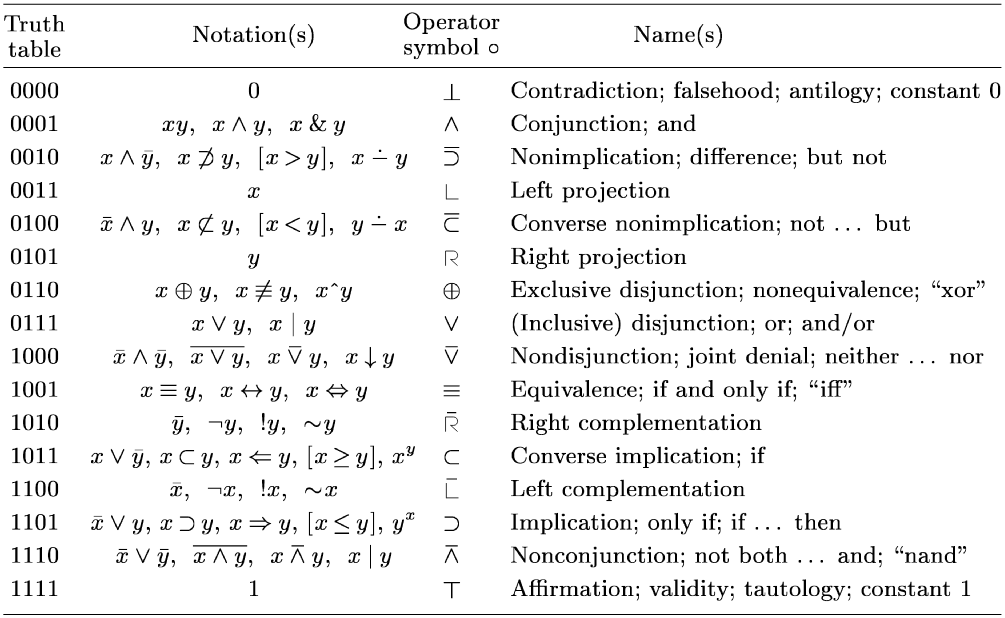
\includegraphics [width=5in]{TableOfPropositionalOperators}
   \caption{TableOfPropositionalOperators}
   \label{table:TableOfPropositionalOperators}
\end{table}

    \subsection {Boolean Expressions and Boolean Functions}

 \begin{table}[htbp]
   \centering
   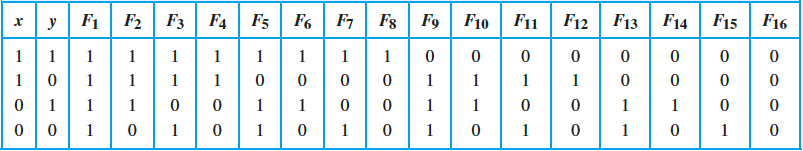
\includegraphics [width=5in]{Table-12-1-3-BooleanFunctionsOfTwoVariables}
   \caption{Table of Boolean Functions of Two Variables}
   \label{table:TableOfBooleanFunctionsOfTwoVariables}
\end{table}

    \subsection {Identities of Boolean Algebra}
    \subsection {Principle of Duality}
Note the similarity of Table 1.1 and 2.1. This is no accident but instead is a fundamental point that is explored in more detail in the math course, Abstract Algebra. One fact that should be noted is the Principle of Duality.

    \subsection {Abstract Definition of a Boolean Algebra}

\section {Representing Boolean Functions}
    \subsection {Sum-of-Products Expansions}
    \subsection {Functional Completeness}
    
\section {Logic Gates}

The logic of signals on wires can be made to obey the laws of logic. Some voltage is used to represent \textit{true} while another is used to represent \textit{false}. Electrical circuits have been created which implement the laws of the logical operators we have already seen and they are called \textit{gates}. We introduce two notations for representing this type of logic, one the visual one which is often seen in a circuits class and another that is a more algebraic notation.

	\begin{definition}[Logic gates]\index{logic gate}

\begin{figure}[htbp]
   \centering
   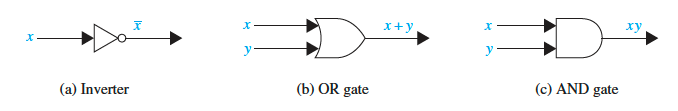
\includegraphics [width=5in]{Figure-12-3-1-BasicGates}
   \caption{Basic Logic Gages}
   \label{figure:BasicLogicGates}
\end{figure}
	\end{definition}

    \subsection {Combinations of Gates}
    \subsection {Adders}
    \subsection {Minimization of Circuits}
	\subsection {combinational circuits versus sequential circuits}
    \subsection {Karnaugh Maps and Quine-McCluskey Method}

Two meanings: one the notation used by Boole, the other the more general observation that this algebra is the same as for logic and sets. The general topic of other algebras is covered in a course on abstract algebra in the math department. 

Sum of Products form for Boolean Algebras
well formed formula
fundamental product
Algorithm for finding sum-of-products form
complete sum of products form, midterms, DNF

Homomorphism between Boolean Algebra and basic logic gates
